% ===== APPENDIX =====
\newpage
\appendix
\section{Appendix}
\label{sec:appendix}

This appendix provides supplementary details that complement the main paper: additional efficiency analyses, reporting notes for statistical testing, small implementation clarifications, and extra qualitative comparisons.

\subsection{Model Architecture Details}
\label{app:model_details}

The following tables show the hyperparameter setup for the pre-training and the downstream fine-tuning for LUNA.

\subsubsection{Hyperparameters for pre-training}
\begin{table}[htbp!]
\centering
\caption{Hyperparameters for EEG pre-training.}
\begin{tabular}{@{}ccccc@{}}
\toprule
\multicolumn{2}{c}{\textbf{Hyperparameters}} & \textbf{LUNA-Base} & \textbf{LUNA-Large} & \textbf{LUNA-Huge} \cr
\midrule
\multirow{5}*{Temporal Encoder} & Input channels & \{1,8,8\} & \{1,16,16\} & \{1,32,32\} \\
& Output channels & \{16,16,16\} & \{24,24,24\} & \{32,32,32\}  \\
& Kernel size & \multicolumn{3}{c}{\{20,3,3\}} \\
& Stride & \multicolumn{3}{c}{\{10,1,1\}} \\
& Padding & \multicolumn{3}{c}{\{9,1,1\}} \\
\midrule
\multicolumn{2}{c}{Patch size} & \multicolumn{3}{c}{40} \\
\multicolumn{2}{c}{Transformer encoder layers} & 8 & 10 & 24 \\
\multicolumn{2}{c}{Number of queries} & 4 & 6 & 8 \\
\multicolumn{2}{c}{Query size} & 64 & 96 & 128 \\
\multicolumn{2}{c}{Hidden size} & 256 & 576 & 1024\\
\multicolumn{2}{c}{MLP size} & 1024 & 2304 & 4096 \\
\multicolumn{2}{c}{Attention head number} & 8 & 12 & 16 \\
\midrule
\multicolumn{2}{c}{Batch size per GPU} & 2040 & 2040 & 720 \\
\multicolumn{2}{c}{Total batch size} & 8160 & 8160 & 11520 \\
\multicolumn{2}{c}{Peak learning rate} & \multicolumn{3}{c}{1.25e-4}\\
\multicolumn{2}{c}{Minimal learning rate} & \multicolumn{3}{c}{2.5e-7} \\
\multicolumn{2}{c}{Learning rate scheduler} & \multicolumn{3}{c}{Cosine} \\
\multicolumn{2}{c}{Optimizer} & \multicolumn{3}{c}{AdamW} \\
\multicolumn{2}{c}{Adam $\beta$} & \multicolumn{3}{c}{(0.9,0.98)} \\
\multicolumn{2}{c}{Weight decay} & \multicolumn{3}{c}{0.05} \\
\multicolumn{2}{c}{Total epochs} & \multicolumn{3}{c}{60} \\
\multicolumn{2}{c}{Warmup epochs} & \multicolumn{3}{c}{10} \\
\multicolumn{2}{c}{Loss type} & \multicolumn{3}{c}{Smooth-L1} \\
\multicolumn{2}{c}{Non-masked region loss coefficient} & \multicolumn{3}{c}{0.05} \\
\multicolumn{2}{c}{Query specialization loss coefficient} & \multicolumn{3}{c}{0.8} \\
\midrule
\multicolumn{2}{c}{Gradient clipping} & \multicolumn{3}{c}{1} \\
\multicolumn{2}{c}{Mask ratio} & \multicolumn{3}{c}{0.5} \\
\multicolumn{2}{c}{Precision} & \multicolumn{3}{c}{bf16-mixed} \\

\bottomrule
\end{tabular}
\label{tab:pre-training}
\end{table}

\clearpage
\subsubsection{Hyperparameters for downstream fine-tuning}

\begin{table}[htbp!]
\centering
\caption{Hyperparameters for downstream fine-tuning.}
\begin{tabular}{@{}cc@{}}
\toprule
\textbf{Hyperparameters} & \textbf{Values} \cr
\midrule
Batch size per GPU & 512 \\
Peak learning rate & 1e-4 \\
Minimal learning rate & 5e-6 \\
Learning rate scheduler & Cosine \\
Optimizer & AdamW \\
Adam $\beta$ & (0.9,0.999) \\
Weight decay & 0.05 \\
Total epochs & 50 \\
Early stopping patience & 10 \\
Warmup epochs & 5 \\
Drop path & 0.1 (B/L) 0.2 (H) \\
Layer-wise learning rate decay & 0.5 (B) 0.8 (L/H) \\
Label smoothing (multi-class classification) & 0.1 \\
\bottomrule
\end{tabular}
\label{tab:finetuning}
\end{table}

\subsubsection{Complexity Analysis}
\label{app:biot_scaling}
The computational complexity of key attention stages and a comparison with alternatives are shown in \ref{tab:app_complexity_breakdown} and 
\ref{tab:app_attention_complexity}.

\begin{table}[htbp!]
\centering
\caption{Complexity Breakdown of LUNA Encoder Stages.}
\label{tab:app_complexity_breakdown}
\begin{tabular}{@{}lcc@{}}
\toprule
\textbf{Stage} & \textbf{Input Shape} & \textbf{Complexity} \\
\midrule
Channel-Unification Module (Cross-Attn) & $(B \cdot S) \times C \times E$ & $O(B \cdot S \cdot Q \cdot C \cdot E)$ \\
Query Self-Attention & $(B \cdot S) \times Q \times E$ & $O(B \cdot S \cdot Q^2 \cdot E)$ \\
Patch-wise Attention Encoder (Self-Attn) & $B \times S \times (Q\cdot E)$ & $O(B \cdot S^2 \cdot Q \cdot E)$ \\ 
\bottomrule
\end{tabular}
\end{table}

\begin{table}[htbp!]
\centering
\caption{Attention Complexity Comparison.}
\label{tab:app_attention_complexity}
\begin{tabular}{@{}lc@{}}
\toprule
\textbf{Method} & \textbf{Bottleneck Complexity} \\ 
\midrule
LUNA (Latent Space Attention) & $O(B \cdot S^2 \cdot Q \cdot E)$ \textit{or} $O(B \cdot S \cdot Q \cdot C \cdot E)$ \\
Full-Attention (e.g., LaBraM) & $O(B \cdot S^2 \cdot C^2 \cdot E)$ \\
Alternating Attention (Patches, e.g., CBraMod) & $O(B \cdot S^2 \cdot C \cdot E)$ \\
Alternating Attention (Channels, e.g., CBraMod) & $O(B \cdot S \cdot C^2 \cdot E)$ \\
\bottomrule
\end{tabular}
\end{table}


\paragraph{BIOT vs.\ LUNA scaling.}
Tables~\ref{tab:biot_patches}--\ref{tab:biot_channels} report GFLOPs and peak activation memory across varying patch and channel counts.

\begin{table}[h]
\centering
\caption{Scaling with patch count (GFLOPs and MiB per forward).}
\label{tab:biot_patches}
\small
\begin{tabular}{lrrrr}
\toprule
Model & \#Patches & FLOPs (G) & Memory (MiB) \\
\midrule
BIOT & 2000 & 1143 & 3534 \\
LUNA-Base & 2000 & 253 & 1835 \\
LUNA-Large & 2000 & 1073 & 2969 \\
LUNA-Huge & 2000 & 6570 & 5549 \\
BIOT & 3000 & 1714 & 5231 \\
LUNA-Base & 3000 & 478 & 3873 \\
LUNA-Large & 3000 & 1886 & 6041 \\
LUNA-Huge & 3000 & 11035 & 9685 \\
BIOT & 4000 & 2286 & 6931 \\
LUNA-Base & 4000 & 768 & 6678 \\
LUNA-Large & 4000 & 2884 & 10265 \\
LUNA-Huge & 4000 & 16286 & 15344 \\
\bottomrule
\end{tabular}
\end{table}

\begin{table}[h]
\centering
\caption{Scaling with channel count (GFLOPs and MiB per forward).}
\label{tab:biot_channels}
\small
\begin{tabular}{lrrrr}
\toprule
Model & \#Channels & FLOPs (G) & Memory (MiB) \\
\midrule
BIOT & 6000 & 3117 & 9270 \\
LUNA-Base & 6000 & 18 & 1571 \\
LUNA-Large & 6000 & 43 & 2410 \\
LUNA-Huge & 6000 & 112 & 4198 \\
BIOT & 7000 & 3637 & 10791 \\
LUNA-Base & 7000 & 20 & 1826 \\
LUNA-Large & 7000 & 49 & 2777 \\
LUNA-Huge & 7000 & 122 & 4680 \\
BIOT & 8000 & 4156 & 12307 \\
LUNA-Base & 8000 & 23 & 2069 \\
LUNA-Large & 8000 & 55 & 3139 \\
LUNA-Huge & 8000 & 133 & 5163 \\
\bottomrule
\end{tabular}
\end{table}

\subsection{Dataset and Preprocessing Details}
\label{app:datasets}

\paragraph{Datasets Used}
We use publicly available EEG datasets,
provided in \ref{tab:app_dataset_summary}.

\begin{table}[htbp!]
\centering
\caption{Summary of Datasets Used.}
\label{tab:app_dataset_summary}
\resizebox{\columnwidth}{!} {
\begin{tabular}{@{}lccccc@{}}
\toprule
\textbf{Dataset} & \textbf{\# Subjects} & \textbf{\# Samples (Train/Val/Test or Total)} & \textbf{Hours of Recordings} & \textbf{\# Channels} & \textbf{Montage Used} \\
\midrule
TUEG (Pre-train) & 14,987 & 15,686,874 (Total) & 21,787.32 & 20 or 22 & Bipolar \\
Siena (Pre-train) & 14 & 101,520 (Total) & 141.0 & 29 & Unipolar \\
TUAB & 2,329 & 591,357 / 154,938 / 74,010 & 1,139.31 & 22 & Bipolar \\
TUAR & 213 & 49,241 / 5,870 / 5,179 & 83.74 & 22 & Bipolar \\
TUSL & 38 & 16,088 / 1,203 / 2,540 & 27.54 & 22 & Bipolar \\
SEED-V & 15 & 43,328 / 43,360 / 31,056 & 32.70 & 62 & Unipolar \\
\bottomrule
\end{tabular}}
\end{table}

\subsection{Experimental Settings}
\label{app:exp_settings}

\paragraph{Pre-training}
LUNA is pre-trained using a masked patch reconstruction task. Key hyperparameters are listed in \ref{tab:pre-training}.

\paragraph{Computational Resources}

Experiments were conducted using NVIDIA A100 GPUs. Pre-training took approximately 1 day on 8 GPUs for the base and large models and 16 GPUs for the huge model.

\subsection{Additional Quantitative Results}
\label{app:quant_extra}

\paragraph{Training Curves}
The pre-training loss curves for LUNA-Base are shown in \ref{fig:app_loss_curve}. The reconstruction loss drops shows and initial plateau then drops slowly over the epochs, while the query specialization shows a jump and then a slow decrease, indicating more orthogonal query usage over time. The initial drop of the query specialization might be due to a trivial case where a query attends to only one channel. The queries learn to attend to their own specialized areas afterwards while covering all the channels in the input.

\begin{figure}[htbp!]
    \centering
    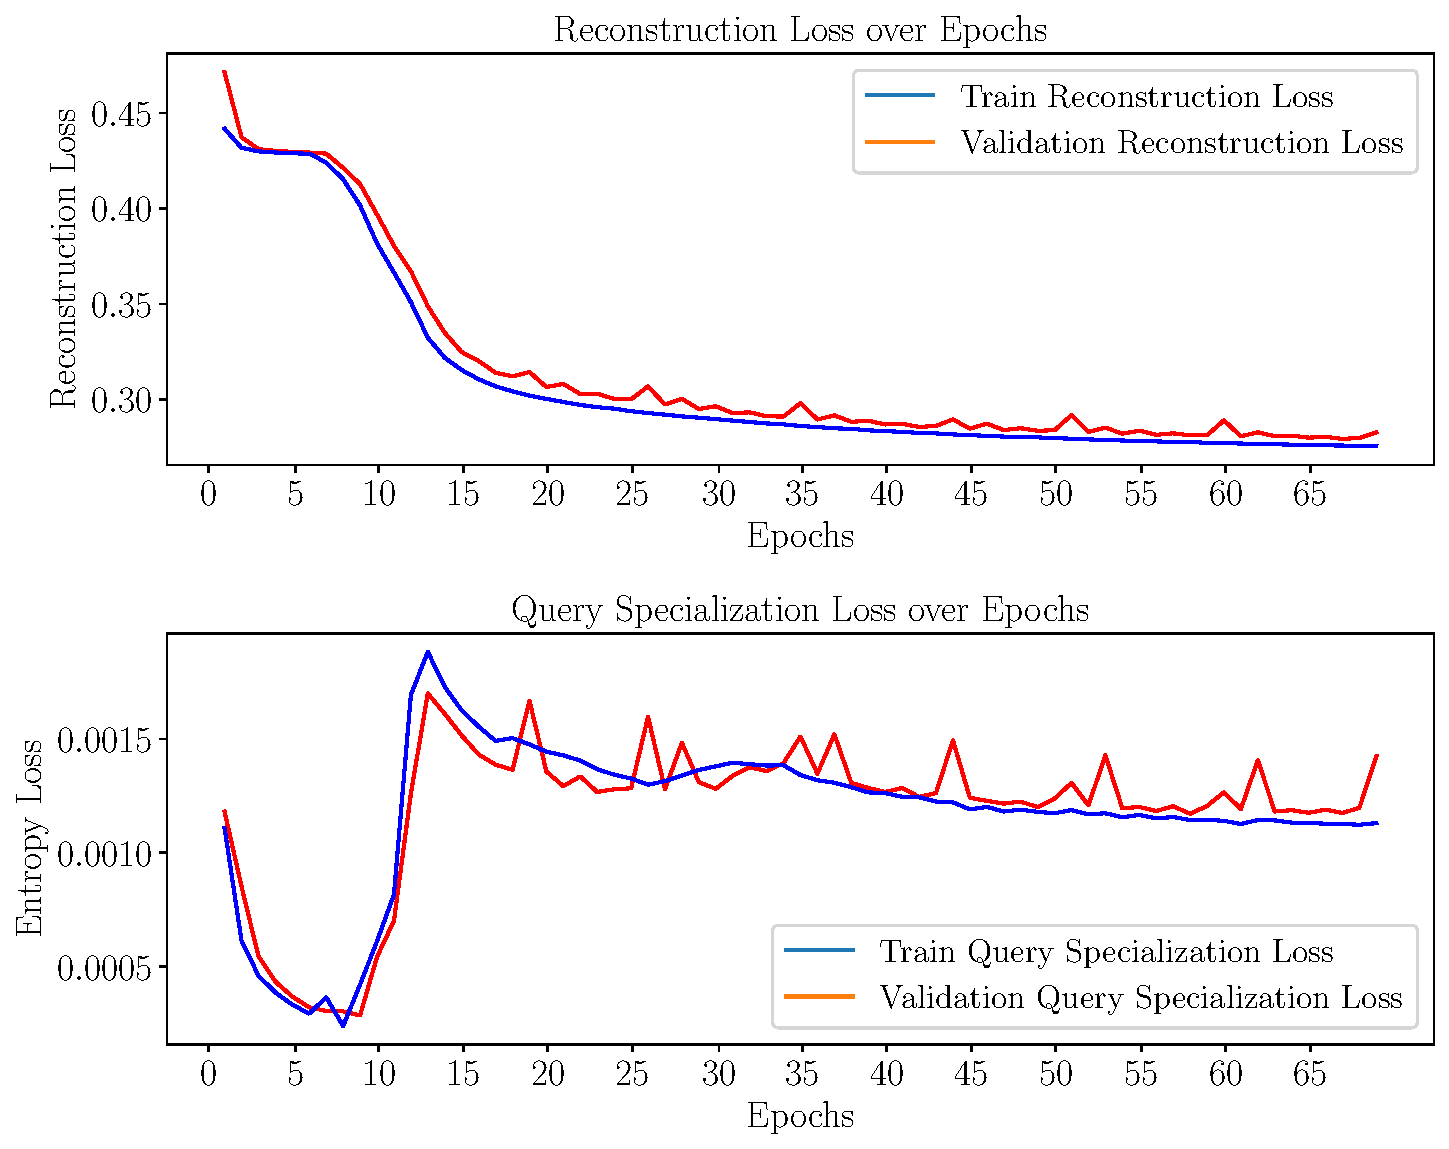
\includegraphics[width=0.8\linewidth]{figs/loss_plot.pdf} 
    \caption{Loss curves during pre-training for LUNA-Base (Reconstruction and Query Specialization Loss).}
    \label{fig:app_loss_curve}
\end{figure}


\subsection{Additional Visualizations}
\label{app:viz_extra}

\paragraph{Reconstruction Examples} 
Figures
\ref{fig:app_20_channels}, \ref{fig:app_22_channels}, \ref{fig:app_29_channels} show examples of the model reconstructing masked patches (gray regions) for inputs with 20, 22, and 29 channels, respectively. The reconstructions capture the underlying signal trend and demonstrate robustness across different topologies seen during pre-training.

\begin{figure}[htbp!]
    \centering
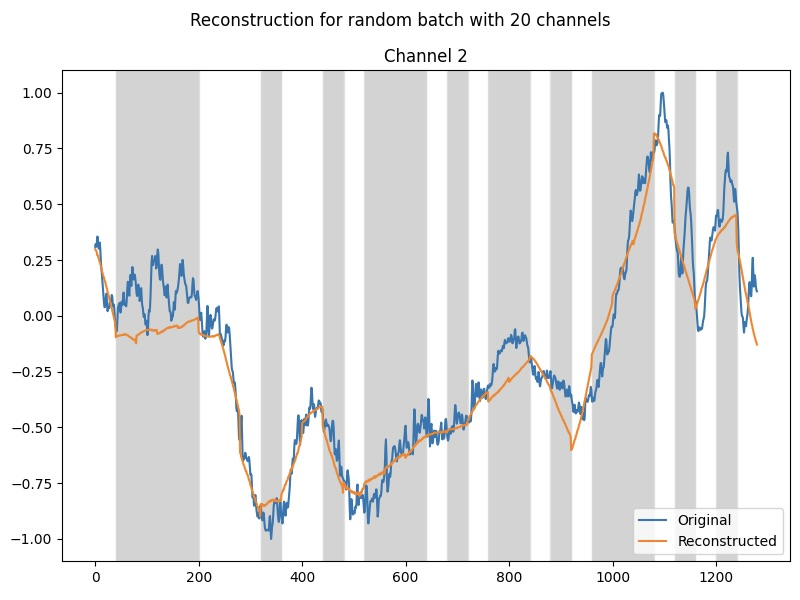
\includegraphics[height=0.25\textheight]{figs/20_chans.jpeg}
    \caption{Example reconstruction on input with 20 channels (masked regions in gray).}
    \label{fig:app_20_channels}
\end{figure}
\begin{figure}[htbp!]
    \centering
    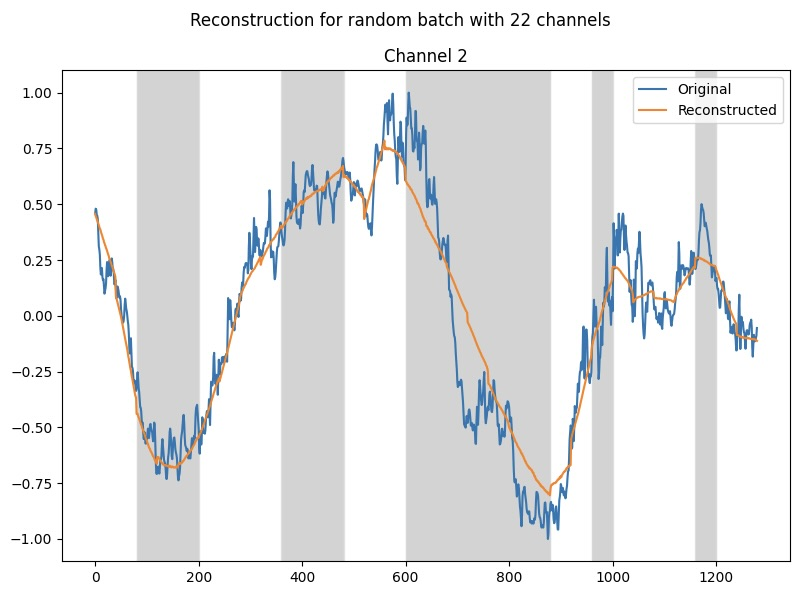
\includegraphics[height=0.25\textheight]{figs/22_chans.jpeg}
    \caption{Example reconstruction on input with 22 channels (masked regions in gray).}
    \label{fig:app_22_channels}
\end{figure}
\begin{figure}[htbp!]
    \centering
    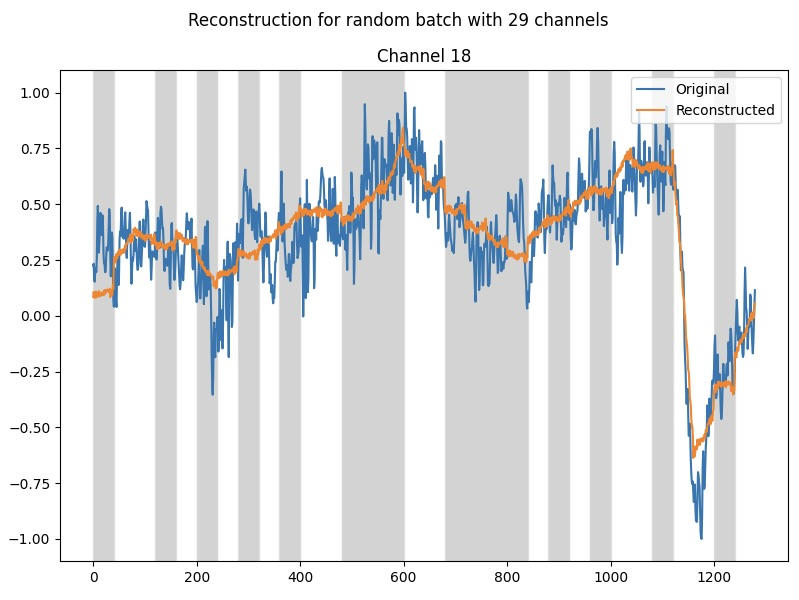
\includegraphics[height=0.25\textheight]{figs/29_chans.jpeg}
    \caption{Example reconstruction on input with 29 channels (masked regions in gray).}
    \label{fig:app_29_channels}
\end{figure}

\subsection{Trade-off between $Q$ and $E$}
\label{app:q_tradeoff}
\begin{table}[h]
\centering
\caption{LUNA-Base variants with fixed $Q\cdot E{=}256$.}
\resizebox{\columnwidth}{!} {
\begin{tabular}{lrrrrrrr}
\toprule
Variant ($Q\times E$) & $Q$ & $E$ & TUAB AUROC & TUAB AUPRC & TUAR AUROC & TUAR AUPRC & TUSL AUROC \\
\midrule
$4\times 64$   & 4  & 64  & 0.887 & 0.895 & 0.902 & 0.495 & 0.767 \\
$2\times 128$  & 2  & 128 & 0.885 & 0.890 & 0.885 & 0.501 & 0.759 \\
$8\times 32$   & 8  & 32  & 0.884 & 0.892 & 0.899 & 0.505 & 0.766 \\
$16\times 16$  & 16 & 16  & 0.874 & 0.881 & 0.866 & 0.487 & 0.757 \\
\bottomrule
\end{tabular}}
\end{table}

\noindent\textit{Observation.} Increasing $Q$ at the expense of $E$ degrades performance; too few queries can also bottleneck capacity. A balanced $Q{\times}E$ (e.g., $4{\times}64$) works well under the same latent budget.

\subsection{Bipolar montage electrode pairs}
\label{app:bipolar_pairs}
We use the following longitudinal pairs to construct the bipolar montage for TUEG, TUAR, TUSL, and TUAB (left/right symmetric sets):
\begin{itemize}\itemsep2pt
  \item Fp1--F7, F7--T3, T3--T5, T5--O1,\quad Fp2--F8, F8--T4, T4--T6, T6--O2 T3--C3, C3--CZ
  \item Fp1--F3, F3--C3, C3--P3, P3--O1,\quad Fp2--F4, F4--C4, C4--P4, P4--O2 CZ--C4, C4--T4
\end{itemize}

\subsection{Edge deployment reference}
Typical low-power edge SoCs used in wearables/IoT offer single-digit to few dozen MB of RAM and on-chip/SiP compute in the 10--100 GOPS range. Under these constraints, LUNA-Base ($\sim$7M params; $\sim$14\,MB at 16-bit) and its measured GFLOPs per window (Fig~\ref{fig:channel_scaling}) fit comfortably within real-time budgets, whereas quadratic-in-$C$ spatial attention and larger activation footprints in some baselines make deployment more challenging at higher channel counts.

\subsection{Significance Testing}
\label{app:sig_tests}
Unless noted, we report mean~$\pm$~s.d.\ over matched seeds. For ablations we ran two-sided paired $t$-tests across seeds for specific comparisons requested by reviewers. For the TUAR AUROC comparison of the model with vs.\ without the query specialization loss, the paired $t$-test yielded $p{=}0.2136$, i.e., not statistically significant at $\alpha{=}0.05$. Observed AUROC deltas across ablations were small (absolute $\le 0.01$).

\begin{table}[h]
\centering
\caption{Paired $t$-test on TUAR AUROC for the specialization-loss ablation.}
\label{tab:sig_tests}
\small
\begin{tabular}{lcc}
\toprule
Comparison & Mean $\Delta$ (w/o $-$ full) & $p$ \\
\midrule
w/o specialization vs.\ full & $-0.007$ & $0.2136$ \\
\bottomrule
\end{tabular}
\end{table}

\paragraph{Practical tolerance.}
We adopt a pragmatic tolerance of $\pm 0.01$ AUROC for considering two variants practically equivalent on these datasets; all reported ablations fall within this band.

\subsection{Effect of Specialization Loss on Query Maps}
\label{app:spec_loss_viz}
Figure~\ref{fig:spec_loss_compare} depicts spatial attention maps of the $Q$ queries when the specialization loss is \emph{removed}. In this setting, two queries converge to coarse lateralized patterns (left and right longitudinal chains), while the remaining queries display broad, overlapping support over fronto–central and midline sites with weaker focal peaks, indicating partial redundancy and gaps in complementary coverage. Overall, the maps exhibit higher overlap and reduced distinctiveness across queries compared to the model trained with the loss, where query maps are more complementary and less overlapping Fig.~\ref{fig:query_analysis}).


\begin{figure}[h]
\centering
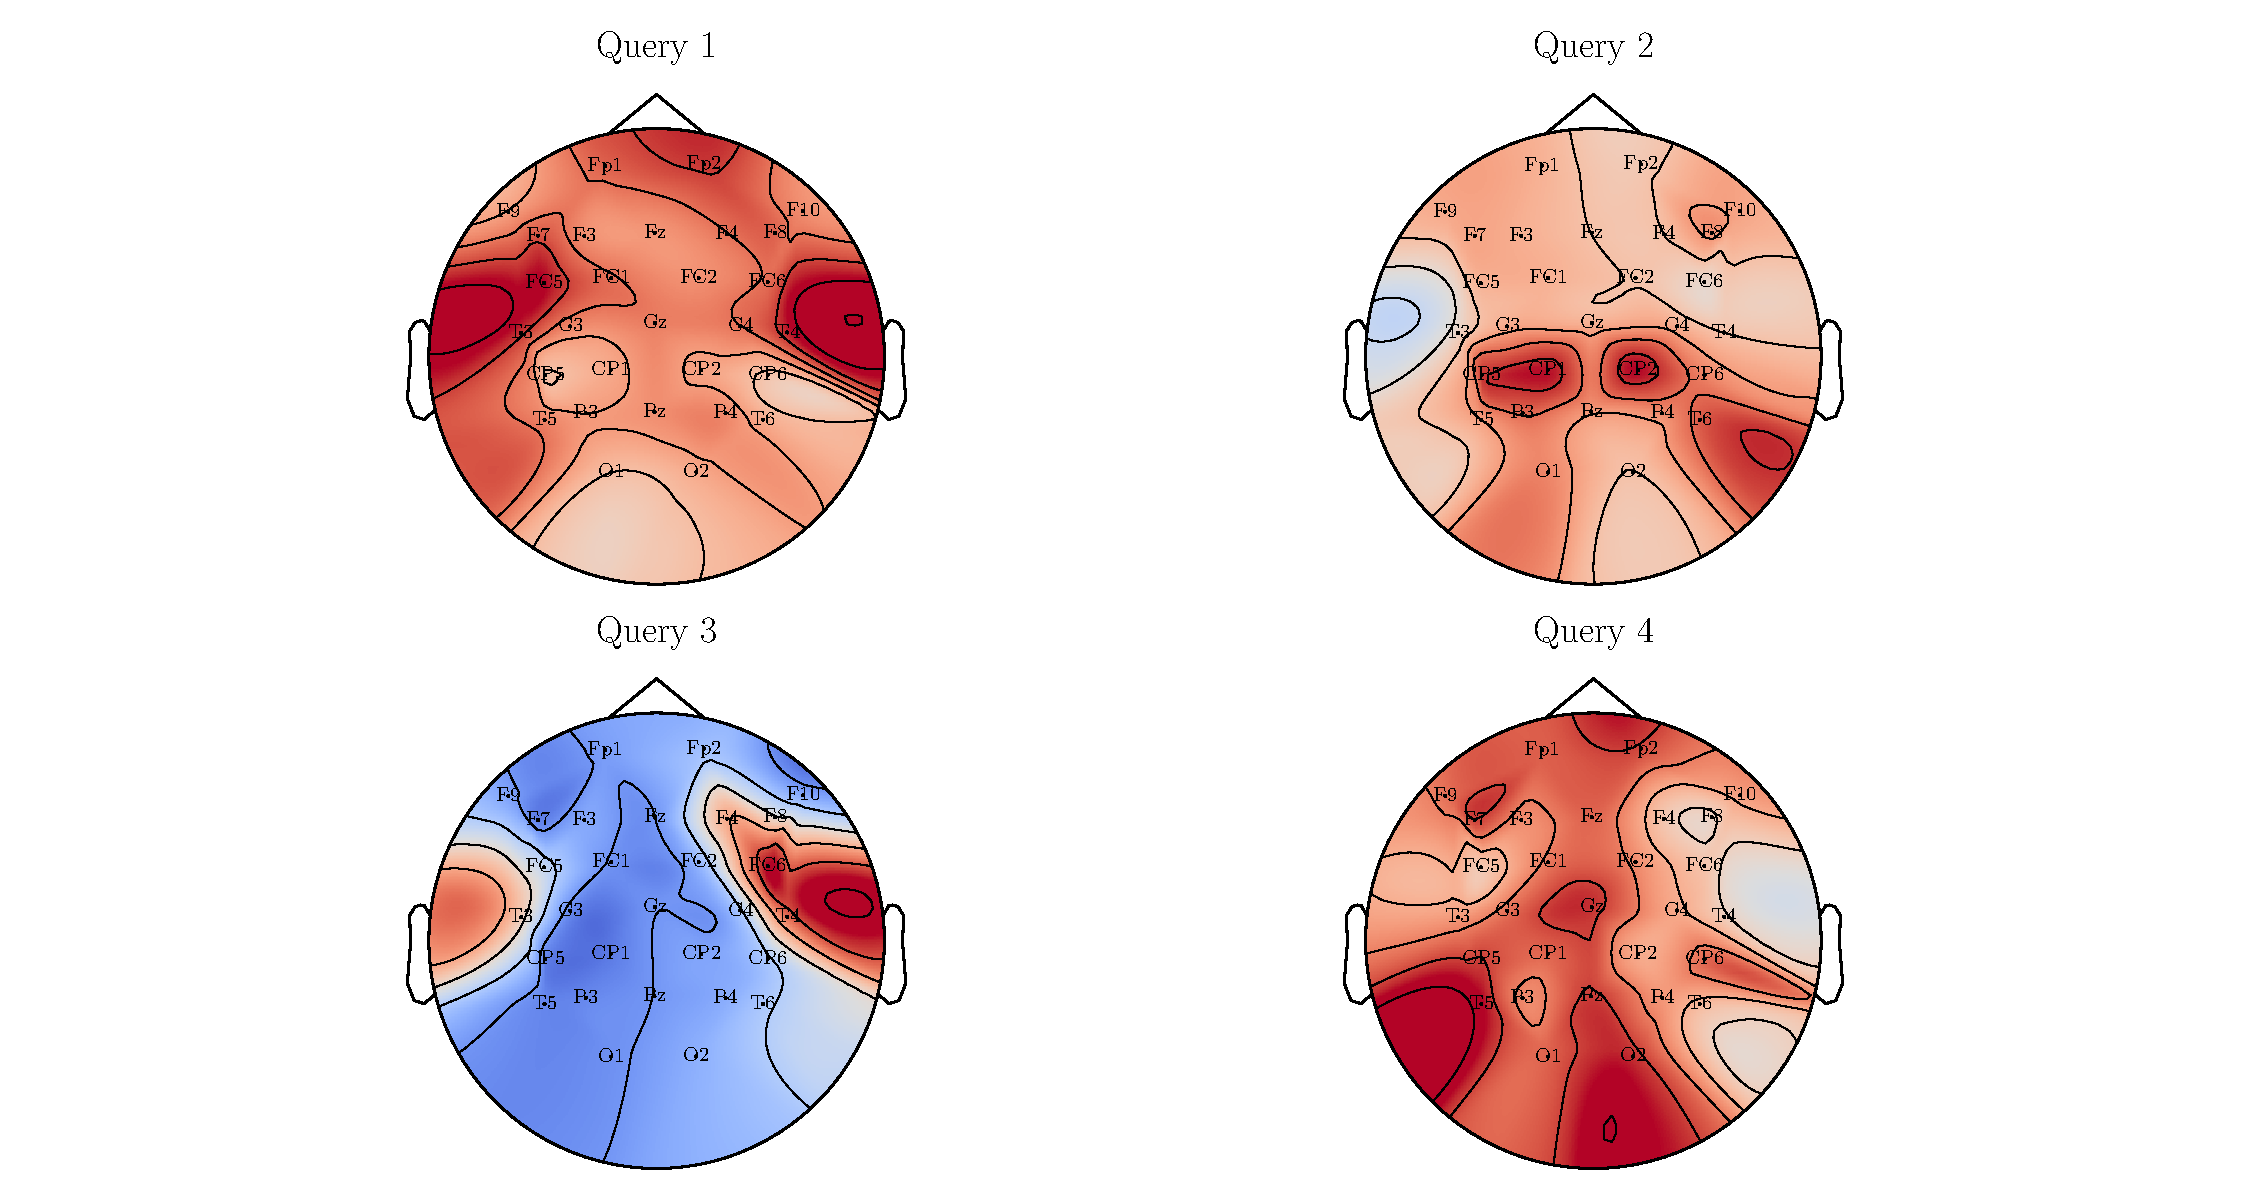
\includegraphics[width=0.95\linewidth]{figs/query_analysis_new.pdf}
\caption{Query attention visualization without specialization loss.}
\label{fig:spec_loss_compare}
\end{figure}

\subsection{t-SNE of Raw Frequency Features vs.\ LUNA Features}
We compute per-segment frequency features (magnitude/phase statistics per band, averaged across channels) and compare 2D t-SNE embeddings to those of LUNA’s latent features. Raw features exhibit less separation beyond clear artifacts on TUAR; LUNA features show tighter clustering aligned with labels.
\begin{figure}[htbp!]
    \centering
    \begin{subfigure}[b]{0.48\textwidth}
        \centering
        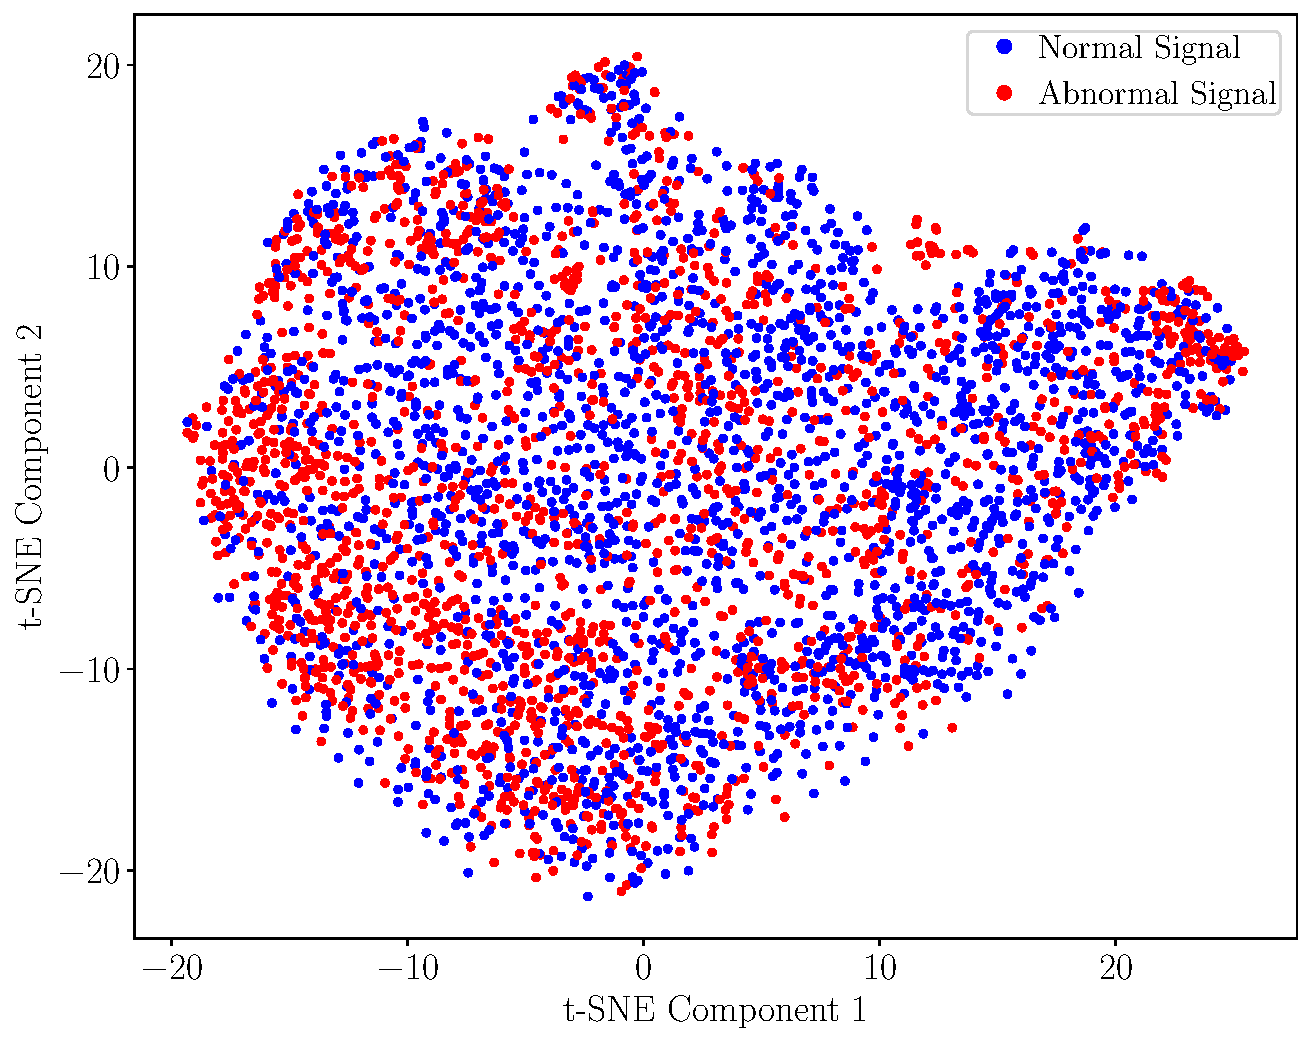
\includegraphics[width=\linewidth]{figs/t-SNE_tuab_new.pdf}
        \caption{TUAB dataset (Normal vs. Abnormal Signal).}
        \label{fig:app_TUAB_emb_raw}
    \end{subfigure}
    \hfill 
    \begin{subfigure}[b]{0.48\textwidth}
        \centering
        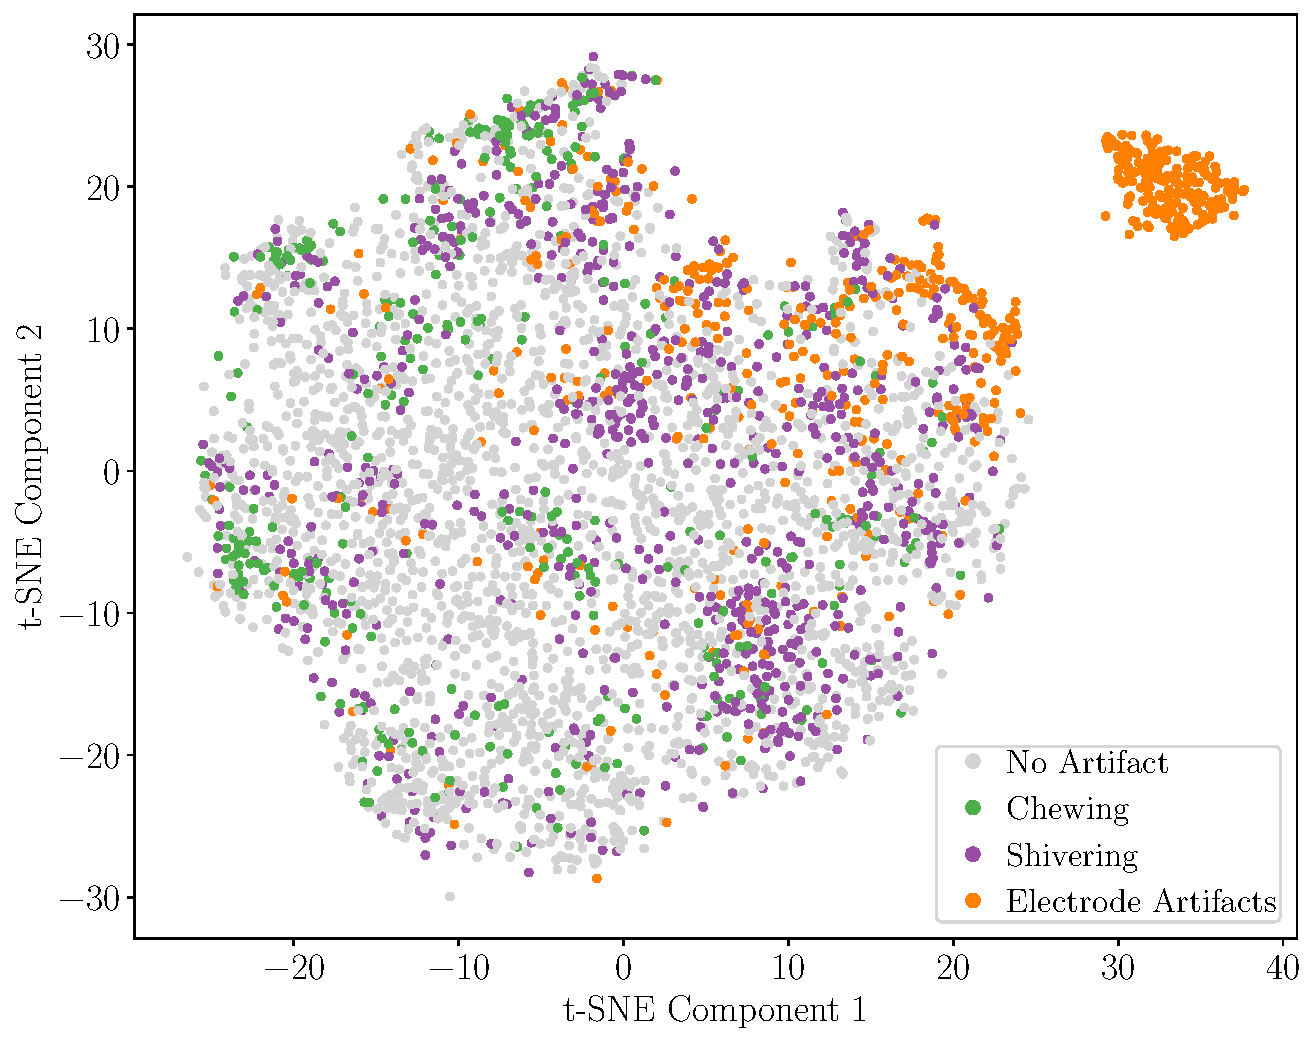
\includegraphics[width=\linewidth]{figs/t-SNE_tuar_new.pdf} 
        \caption{TUAR dataset (Artifact Types).}
        \label{fig:app_TUAR_emb_raw}
    \end{subfigure}
    \caption{t-SNE of raw features on downstream datasets before fine-tuning.}
    \label{fig:t-sne-raw}
    \vspace{-0.5cm}
\end{figure}



% ===== END APPENDIX =====